\section{Itération 0 }



\subsection{Objectif de l'itération }
Avant de commencer la première itération du Scrum, une période de temps à été
consacrée pour préparer ce qui est nécessaire au lancement du projet dans de bonnes
conditions. cette période est souvent nommé l’itération 0 du projet. Elle est consacrée
généralement à la recherche bibliographique, aux choix technologiques et à la mise en
place de l’environnement de développement. Outre que ces préparatifs, c’est dans cette
itération que nous définissons le Backlog de la Plateforme, ainsi que le nombre
d’itérations nécessaires et la durée de l’itération. Il s’agit aussi d’une période de
formation pour les membres de l’équipe sur tous les environnements et les technologie à
utiliser au cours du montage du produit.

\begin{figure}[htbp]
  \centering
  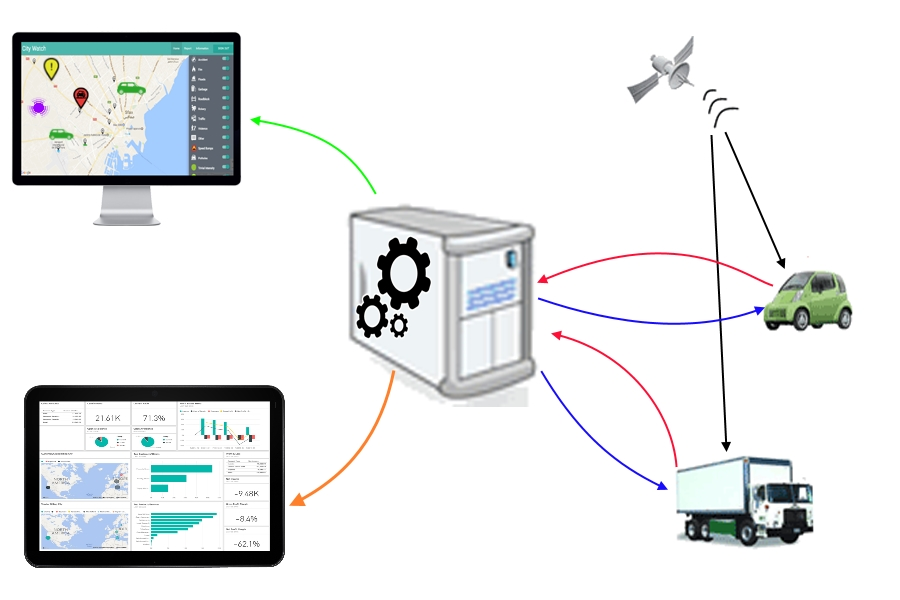
\includegraphics[width=0.8\textwidth]{citywatch-architecture}
  \caption[Flux des information Géographiques en CityWatch]
  {Flux des informations Géographiques dans le systéme de tracking de la plateforme CityWatch}
  \label{fig:citywatch-architecture}
\end{figure}
\subsection{Backlog générale}

La première étape de la méthode Scrum consiste à préparer un carnet du produit
(Product Backlog) qui présente la liste des tâches à effectuer durant le développement
du projet qui sera répartie en des itérations. Le rôle du product-owner est important
dans cette phase de développement parce qu’il devra faire l’exercice de prioriser ses
demandes selon des critères respectant la mission et les objectifs de son produit. En
précisant la valeur de priorité, il estime l’impact et le retour sur investissement 
qu’aura chacun des items dans le carnet du produit.
Il y a donc effectivement eu un gros travail
d’échanges et discussions avec le client pour comprendre tout le cahier des charge
initial,C’est comme ça que le Backlog a été défini.

La figure~\ref{fig:product-backlog} présente une version simplifié du product
backlog décrit dans le tableau~\ref{tab:product-backlog}.
%\usepackage{dtklogos}
\usetikzlibrary{mindmap,shadows}
% Information boxes
\newcommand*{\info}[4][16.3]{%
  \node [ annotation, #3, scale=0.65, text width = #1em,
          inner sep = 2mm ] at (#2) {%
  \list{$\bullet$}{\topsep=0pt\itemsep=0pt\parsep=0pt
    \parskip=0pt\labelwidth=8pt\leftmargin=8pt
    \itemindent=0pt\labelsep=2pt}%
    #4
  \endlist
  };
}
\begin{tikzpicture}[every annotation/.style={draw, fill=white, font=\Large}]
    \renewcommand{\href}[2]{#2}

    \path[mindmap,
          concept color=black!40,
          text=white,
          every node/.style={
              concept,
              circular drop shadow,
              execute at begin node=\hskip0pt,
          },
          %grow cyclic,
          root/.style={
              concept color=black!40,
              fill=white, line width=1ex, text=black,
              font=\footnotesize\bfseries,
              text width=7em},
          level 1 concept/.append style={
              font=\normalsize\bfseries,
              sibling angle=50,
              text width=7.7em,
              level distance=12.5em,
              inner sep=0pt},
          level 2 concept/.append style={
              font=\footnotesize\bfseries,
              level distance=8em},
    ]

    node[root] {Platforme CityWatch} [clockwise from=0]
    child[concept color=blue!60] {
        node {Gestions des Rapports} [clockwise from=90]
        child { node (goForum) { Consultation } }
        child { node (goWiki) { Déclaration } }
    }
    child[concept color=blue] {
        node[concept] {Systeme de protection }
        [clockwise from=30]
        child { node[concept] (TeXnique)
            { Alert Secousses} }
        child { node[concept] (TeXweltQA)
            { Alert Doudannes} }
        child [faded] { node[concept] (TeXweltBlog)
            { Dedaction }}
    }
    child[concept color=green!40!black] {
        node[concept] {\href{http://texample.net/}{\TeX ample\\.net}}
        [clockwise from=310]
        child { node[concept] (TikZGalerie)
            {\href{http://texample.net/tikz/examples/}{TikZ-Galerie}} }
        child { node[concept] (TeXampleBlog)
            {\href{http://texample.net/weblog/}{Blog}} }
        child { node[concept] (Planet)
            {\href{http://texample.net/community/}{Planet}} }
    }
    child[concept color=red] {
        node[concept] (PGFPlots) {\href{http://pgfplots.net}{PGFPlots\\.net}}
        [clockwise from=270]
    }
    child[concept color=red!60!black] {
        node[concept] {\href{http://latex-community.org/}{\LaTeX-Community\\.org}}
        [counterclockwise from=100]
        child { node[concept] (LaTeXForum)
            {\href{http://latex-community.org/forum/}{Forum}}}
        child { node[concept] (LaTeXArtikel)
            {\href{http://latex-community.org/know-how}{Artikel-Archiv}} }
        child { node[concept] (LaTeXNews)
            {\href{http://latex-community.org/home/news}{News}} }
    }
    child[concept color=orange] {
        node[concept] (TeXdoc)
        {\href{http://texdoc.net/}{\TeX doc\\.net}}
        [clockwise from=100]
        child { node[concept] {\href{http://www.tex.ac.uk}{UK \TeX \\FAQ}}
        }}
    child[concept color=yellow!60!black] {
        node[concept] (Blogs) {Blogs} [clockwise from=139]
        child { node[concept] {\href{http://texblog.net/}{\TeX blog\\.net}}}
        child { node[concept] {\href{http://tikz.de/}{TikZ.de}} }
        child { node[concept] (Cookbook)
            {\href{http://latex-cookbook.net/}{\LaTeX-\\Cookbook\\.net}} }
    };
    %\info{goForum.north east}{above,anchor=west,xshift=1em}{%
    %  \item[] Seit 2008
    %  \item 68\,444 Beiträge
    %  \item 13\,715 Themen
    %  \item 5\,532 registrierte Nutzer
    %}
    %\info{LaTeXForum.north west}{above,anchor=south}{%
    %  \item[] Seit 2008
    %  \item 81\,991 Beiträge
    %  \item 21\,026 Themen
    %  \item 13\,354 registrierte Nutzer
    %}
    %\info[8]{LaTeXArtikel.west}{below,anchor=north east,xshift=3em,yshift=-2em}{%
    %  \item 115 Artikel
    %}
    %\info[11]{LaTeXNews.south west}{below,anchor=north}{%
    %  \item 240 Meldungen
    %}
    %\info[9]{TikZGalerie.south}{below,anchor=north}{%
    %  \item[] Seit 2006
    %  \item 172 Autoren
    %  \item 384 Beispiele
    %}
    %\info[15]{goWiki.south}{below,anchor=north,xshift=3em}{%
    %  \item 152 erklärte Konzepte, Befehle und Pakete
    %}
    %\info{TeXweltQA.south east}{above,anchor=north west}{%
    %  \item[] Seit 2013
    %  \item 1\,710 Fragen
    %  \item 2\,151 Antworten
    %  \item 479 registrierte Nutzer
    %}
    %\info[8]{TeXweltBlog.south}{below,anchor=north,xshift=2em}{%
    %  \item[] Seit 2013
    %  \item 14 Autoren
    %}
    %\info[9]{PGFPlots.south west}{anchor=north east,xshift=1em}{%
    %  \item 14 Autoren
    %  \item 59 Beispiele
    %}
    %\info[6]{Planet.west}{anchor=east}{%
    %  \item 46 Blogs
    %}
    %\info[14]{TeXnique.east}{anchor=west,xshift = 0.5em}{%
    %  \item[] 2015, aufgrund Idee mit französischen
    %          \TeX-Freunden nach der TUG Damstadt, experimentell
    %}
    %\info[16]{Cookbook.east}{anchor=south west}{%
    %  \item[] Ab 10/2015, soll ca. 100 Beispiele aus
    %          dem \LaTeX\ Cookbook zeigen, sowie
    %          Community-Rezepte
    %}
\end{tikzpicture}


\begin{center}
    \footnotesize
    \setlength\LTleft{-50pt}
\begin{longtable}{| l | p{3.5cm} | l | p{4.5cm} | p{4.5cm} | l |}
 \caption{Product Backlog}
 \label{tab:product-backlog} \\

 \hline
 \textbf{ID} & \textbf{Cas d'utilisations} & \textbf{En tant qu'} & \textbf{Je veux qu'} & \textbf{Pour} & \textbf{Priorité} \\ \hline
 \endhead

 \hline \multicolumn{6}{|r|}{{Continué en page suivante$\dotsc$}} \\ \hline
 \endfoot

 \hline \hline
 \endlastfoot

\hline
 1 & Gestion du Trajectoire & Utilisateur & Il soit possible de démarrer le tracking & Avoir un feedback dans l'application et sur le site web & 1 \\
   &                        & Utilisateur & Il soit possible d’arrêter le tracking & Avoir un feedback dans l’application & 1 \\ \hline
 2 & Gestion de Rapports    & Utilisateur & Il soit possible de choisir entre une variété de problèmes à déclarer depuis l’application & Avoir un feedback sur le site web & 1 \\
   &                        & Utilisateur & Il soit possible de choisir l’emplacement du problème à déclarer dans une carte & Avoir un feedback sur le site web & 1 \\
   &                        & Utilisateur & Il soit possible d’ajouter une description ou une image au problème & Avoir un feedback sur le site web & 2 \\ \hline
 3 & Consulter la carte     & Utilisateur & Il soit possible de consulter la carte depuis l’application & Voir la carte dans l’application & 2 \\ \hline
 4 & Compte                 & Utilisateur & Il soit possible de consulter le site web sans avoir un compte & Consulter le site web avec un minimum d’informations & 1 \\
   &                        & Utilisateur & Il soit possible de créer un compte & Avoir un compte personnel & 2 \\ \hline
 5 & Groupement des rapports& Utilisateur & Il est possible de voir les rapports en groupe lors d’un zoom out & Avoir une vision globale sur le nombre des rapports & 1 \\ \hline
 6 & Déclarer un rapport    & Utilisateur & Il est possible de déclarer un rapport à partir du site web & Avoir accès à une page rapport comme celle de l’application & 1 \\ \hline
\end{longtable}
\end{center}
\subsubsection{Modélisation UML}
\subsection{Préparation de l'environnement du travail}
\subsubsection{Environnement logiciel}
La réalisation de ce projet nécessite l’ensemble de ces logiciels et bibliothèques :
\paragraph{Android studio}
\TODO{description}
\paragraph{PHPStorm}
il est un environnement de développement intégré (IDE) dédié pour la
programmation en PHP. Il regroupe sous une interface conviviale un éditeur de texte, un
interpréteur et un débogueur.... Ceci permet de faciliter la tâche de programmation et de
maximiser la productivité des développeurs.
\TODO{description}
\paragraph{VIM}
\paragraph{Composer}
\subsubsection{environnements matériels}
Pour le développement de ce projet il était demandé d’avoir :
\begin{itemize}
 \item Serveur Local pour les tests
 \begin{itemize}
     \item Windows 10
     \item Wamp 5
     \item Apacje2.?
     \item PHP 7.0
     \item MySQL 5 
 \end{itemize}
 \item Serveur Production: 
 \begin{itemize}
  \item Linux
  \item Access FTP
  \item Apache 2.? \TODO{2.XXXXX}
  \item  PHP 7
  \item  MySQL
 \end{itemize}
\end{itemize}

\subsection{Conclusion}

L’itération 0 à permis de préparer le terrain pour une bonne entame de
développement. Mis à part la mise en place des environnement de travail et les
formations que nous avons suivi sur les technologies, cette itération a permis d’élaborer
le carnet de Plateforme CityWatch avec la collaboration du product owner et de fixer le
nombre des itérations et leur durée. Rappelons que l’itération 0 à durée trois jours,
du 20 février 2017 au 22 février 2017.
